\documentclass[conference]{IEEEtran}
\IEEEoverridecommandlockouts
% The preceding line is only needed to identify funding in the first footnote. If that is unneeded, please comment it out.
\usepackage{cite}
\usepackage{amsmath,amssymb,amsfonts}
\usepackage{algorithmic}
\usepackage{graphicx}
\usepackage{url}
\usepackage{caption}
\usepackage{float}
\usepackage{hyperref}\usepackage{adjustbox}
\usepackage{array}

\newcolumntype{R}[2]{%
    >{\adjustbox{angle=#1,lap=\width-(#2)}\bgroup}%
    l%
    <{\egroup}%
}
\newcommand*\rot{\multicolumn{1}{R{90}{-1em}}}% no optional argument here, please!

\def\BibTeX{{\rm B\kern-.05em{\sc i\kern-.025em b}\kern-.08em
    T\kern-.1667em\lower.7ex\hbox{E}\kern-.125emX}}
\begin{document}

\title{Predicting Bitcoin Price using LSTM and Twitter Sentiment Analysis\\
%{\footnotesize \textsuperscript{*}Note: Sub-titles are not captured in Xplore and
%should not be used}
%\thanks{Identify applicable funding agency here. If none, delete this.}
}

\author{\IEEEauthorblockN{}
\IEEEauthorblockA{\textit{Haruki Moriguchi} \\
\textit{haruki.moriguchi@mail.mcgill.ca} \\
ID: 260665818}
\and
\IEEEauthorblockN{}
\IEEEauthorblockA{\textit{Edwin H.Ng} \\
\textit{edwin.ng@mail.mcgill.ca} \\
ID: 260732345}
}

\twocolumn[
  \begin{@twocolumnfalse}
    \maketitle
    \begin{center}
    \begin{minipage}{0.5\linewidth}
    \begin{abstract}
	\textbf{The prediction of stock markets have posed serious challenges to researchers since many factors such as political events, the public opinion and the market trend influence the stock prices. The objective of this paper is to consider a Long Short-Term Memory (LSTM) neural network ensemble that predicts the future prices of Bitcoin based on the historical prices of Bitcoin, the volume of tweets related to Bitcoin as well as the sentiment analysis of these tweets. These represent the trend of the Bitcoin price, its popularity, and the public opinion about it, respectively. LSTM has the advantage of creating dependencies between data that are arbitrarily far apart, and an LSTM ensemble combines the multiple forecast results from a set of individual LSTM networks consisting of the initial forecast of the price of Bitcoin, the forecast of the volume of tweets, and the sentiment analysis of the latter in order to output a final prediction for the price of Bitcoin.}
\end{abstract}
\begin{IEEEkeywords}
\begin{center}
\textbf{Bitcoin, LSTM, Sentiment Analysis, word2vec}
\end{center}
\end{IEEEkeywords}
    \end{minipage}
    \end{center}
  \end{@twocolumnfalse}
]

\section{Introduction}
\par In recent years, Bitcoin has gained enormous popularity. After receiving many media coverage in 2017, the price went up drastically from 1,000 to 20,000 USD, from which it has since gone down. In fact, this sudden increase in price is not surprising, since behavioral economics states that there are correlations between the public sentiment and the financial market. Fortunately, with the advent of social media, the information about public feelings has become abundant, where Twitter has received a lot of attention from researchers.
\par The primary contributions of this paper is to test the hypothesis that, in addition to past historical prices, the public sentiment also influences the market. The idea is that although the future movement of a stock price should be a reflection of its past tendencies, the public opinion should also be of important influence to its trajectory. In fact, high pessimism toward a stock should be followed by a downward movement and high optimism should be followed by an upward movement. 
\par The proposed approach is structured as follows. First, a sentimental analysis is performed on Bitcoin tweets where they are labelled as "negative" or "positive" according to a LSTM classifier. Two other LSTMs are used as time series models to forecast the price of Bitcoin, and the volume of tweets respectively. The outputs of the sentiment analysis of the tweets, the prediction of their volume, and the predicted price of the Bitcoin are then combined together to form a LSTM ensemble that predicts a final price for the Bitcoin. That is, the initial forecast of the Bitcoin price is fine-tuned with additional information provided by the volume and the sentiment of tweets. The idea is that although an assets should reflect its past historical prices, its growing popularity among the public and their sentiment towards it should also impact its future price.
\par The data consists of 2,564,353 tweets related to Bitcoin ranging from October 31, 2017 till November 27, 2017. The Bitcoin price data consists of the hourly prices matching with the corresponding time period.
	 
 % ------------------------
\section{Related Work}
\par Prediction of stock markets has been proven to be complex and challenging since they are by nature very stochastic. On the one hand, the Efficient-Market hypothesis states that the current price of an asset should be a reflection of all its previous information. On the other hand, the Random-Walk hypothesis claims that the price is independent of its history. Nonetheless, many researchers agree that the prediction of stock markets can be achieved to some degree.  
\par Recently, the LSTM neural network has gained popularity where it has been used by Nelson et al. \cite{LSTM Stock} to predict the future movement of stock prices. In fact, LSTM has gained notoriety as a time series model, since it can maintain contextual information as well as temporal behaviours of events. In particular, Zhuge et al. \cite{LSTM Emotional} use the LSTM as a time series model to predict the Shanghai Composite Index based on its historical prices. Furthermore, they incorporate an emotional market data into their model in order to reflect the influence of the public opinion on the stock market. The emotional data was obtained through a sentiment analysis based on a Naive Bayes Classifier that was fed with posts text from Eastmoney with regard to the stocks. Similarly, Khedr et al. \cite{Behavior} consider predicting the stock movement through a KNN algorithm that takes into account both its historical prices and the output of a sentiment analysis based on a Naive Bayes Classifier applied to Reuter news. 
\par Another popular source of public opinion is Twitter. In the context of predicting the stock movement through public sentiment, Pagola et al. \cite{word2vec Twitter} introduce the use of word2vec in order to textually represent the tweets, whereas the classical approach would be to use the N-gram representation. The former allows for sustainability in word meaning across different contexts.
\par The contribution of this paper is to consider a LSTM ensemble that combines the sentiment analysis of Bitcoin tweets, the forecasts of its volume and the initial forecasts of the Bitcoin prices in order to predict a final price for the Bitcoin. The initial forecasts of the price of Bitcoin and of the volume of tweets are performed through a LSTM acting as a time series model. The sentiment analysis of the tweets is assessed through another LSTM model, and a word2vec modelling is used to assess the feature vector representations of the tweets. Several authors \cite{LSTM Ensemble 1} have demonstrated the effective use of a LSTM ensemble. 

 % ------------------------
\section{Method}

\subsection{Data Collection}
\par The closing prices of Bitcoin have been extracted hourly from October 31, 2017 till November 27, 2017 \footnote{\url{https://bitcoincharts.com}}. Figure \ref{Bitcoin Price} shows the price going in an upward trend from \$6,123.21 to \$9,328.25. It is interesting to note that the trend of the volume of tweets, shown in figure \ref{Bitcoin Volume Tweets}, is increasing over that same period as well, suggesting a correlation between the price and the volume of tweets. The volume of tweets is extracted from the following data. A total of 2,424,480 tweets related to Bitcoin over the period  of October 31, 2017 till November 27, 2017 are extracted from the Twitter API \cite{Twitter API}, using keywords like \# Bitcoin, \# BTC, \# Cryptocurrency, \# Cryptos, etc. 

\begin{minipage}{\linewidth}
\begin{figure}[H]
\centering
\caption{Bitcoin Price from October 31, 2017 till November 27, 2017} 
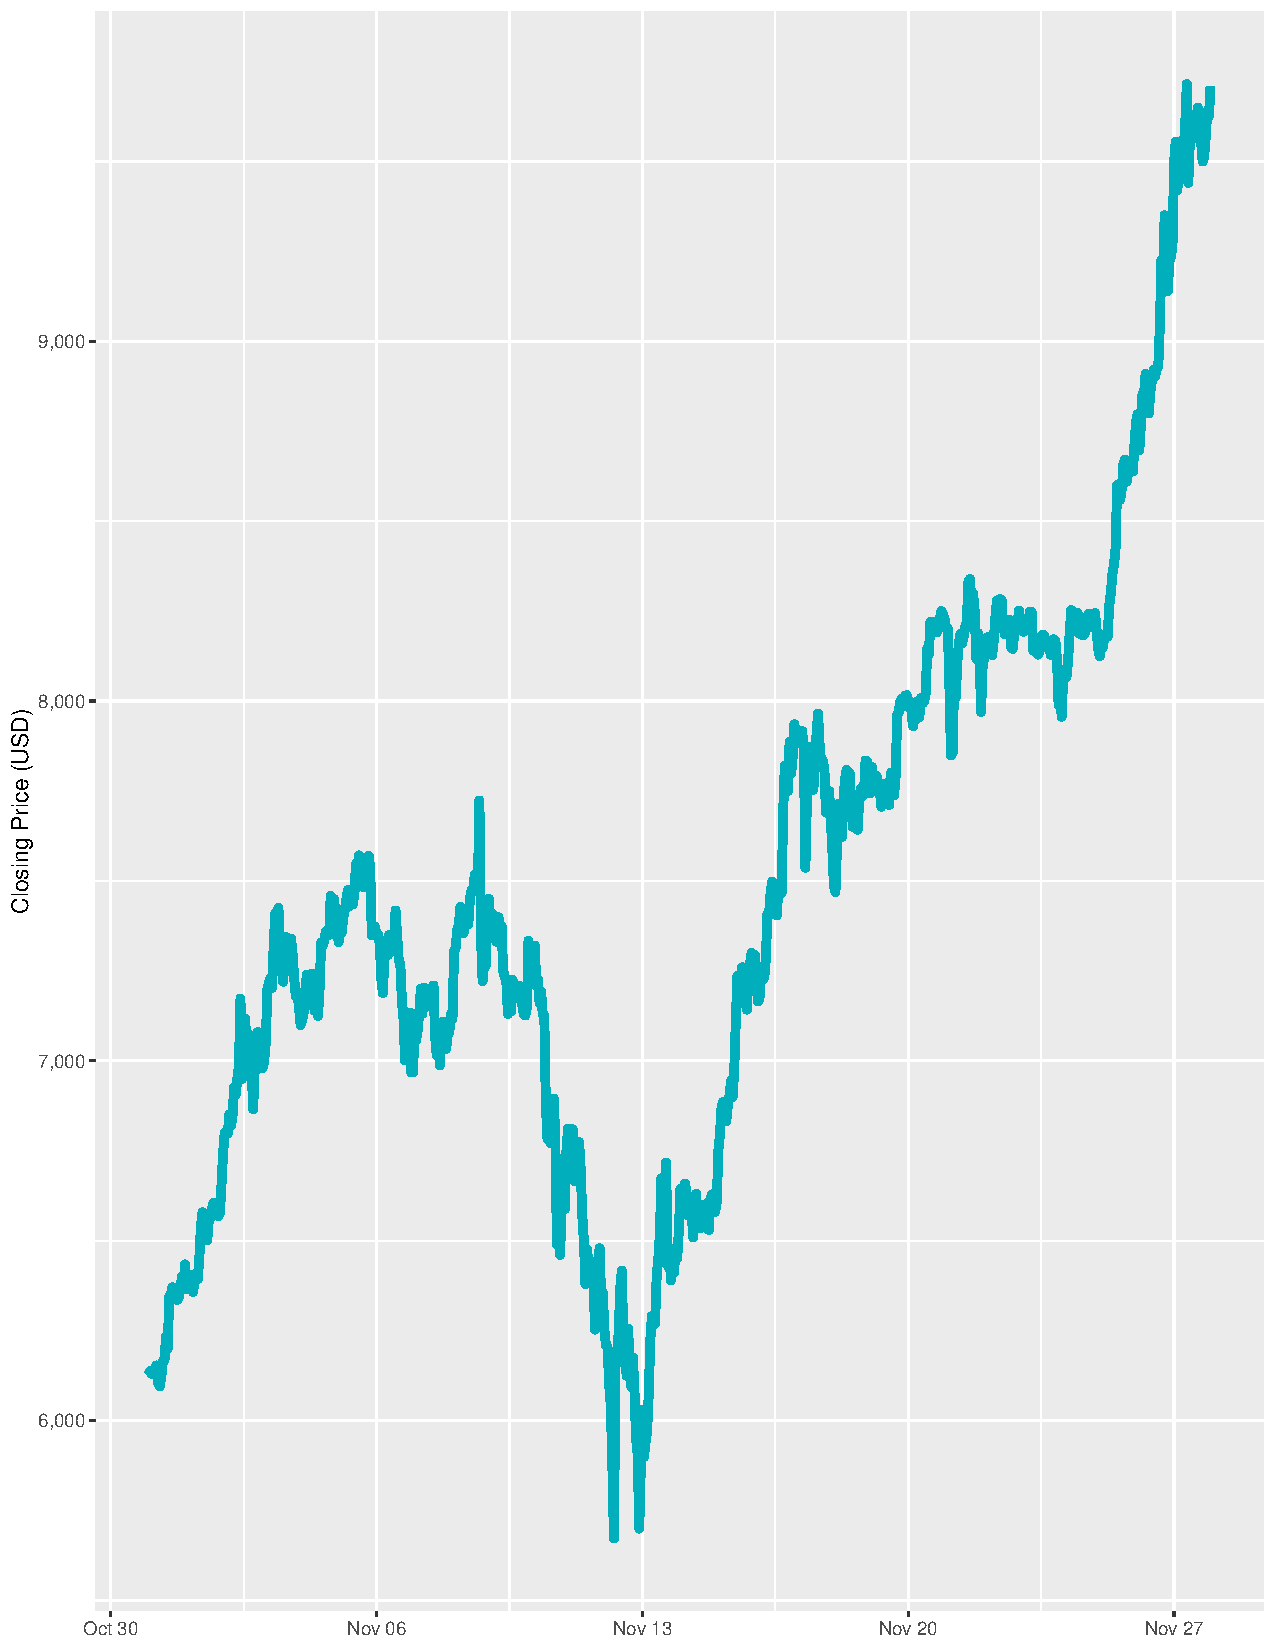
\includegraphics[scale=0.3]{Graphs/BitcoinPriceChart.pdf}
\label{Bitcoin Price} 
\end{figure}
\end{minipage}

\begin{minipage}{\linewidth}
\begin{figure}[H]
\centering
\caption{Bitcoin Volume Tweets from October 31, 2017 till November 27, 2017} 
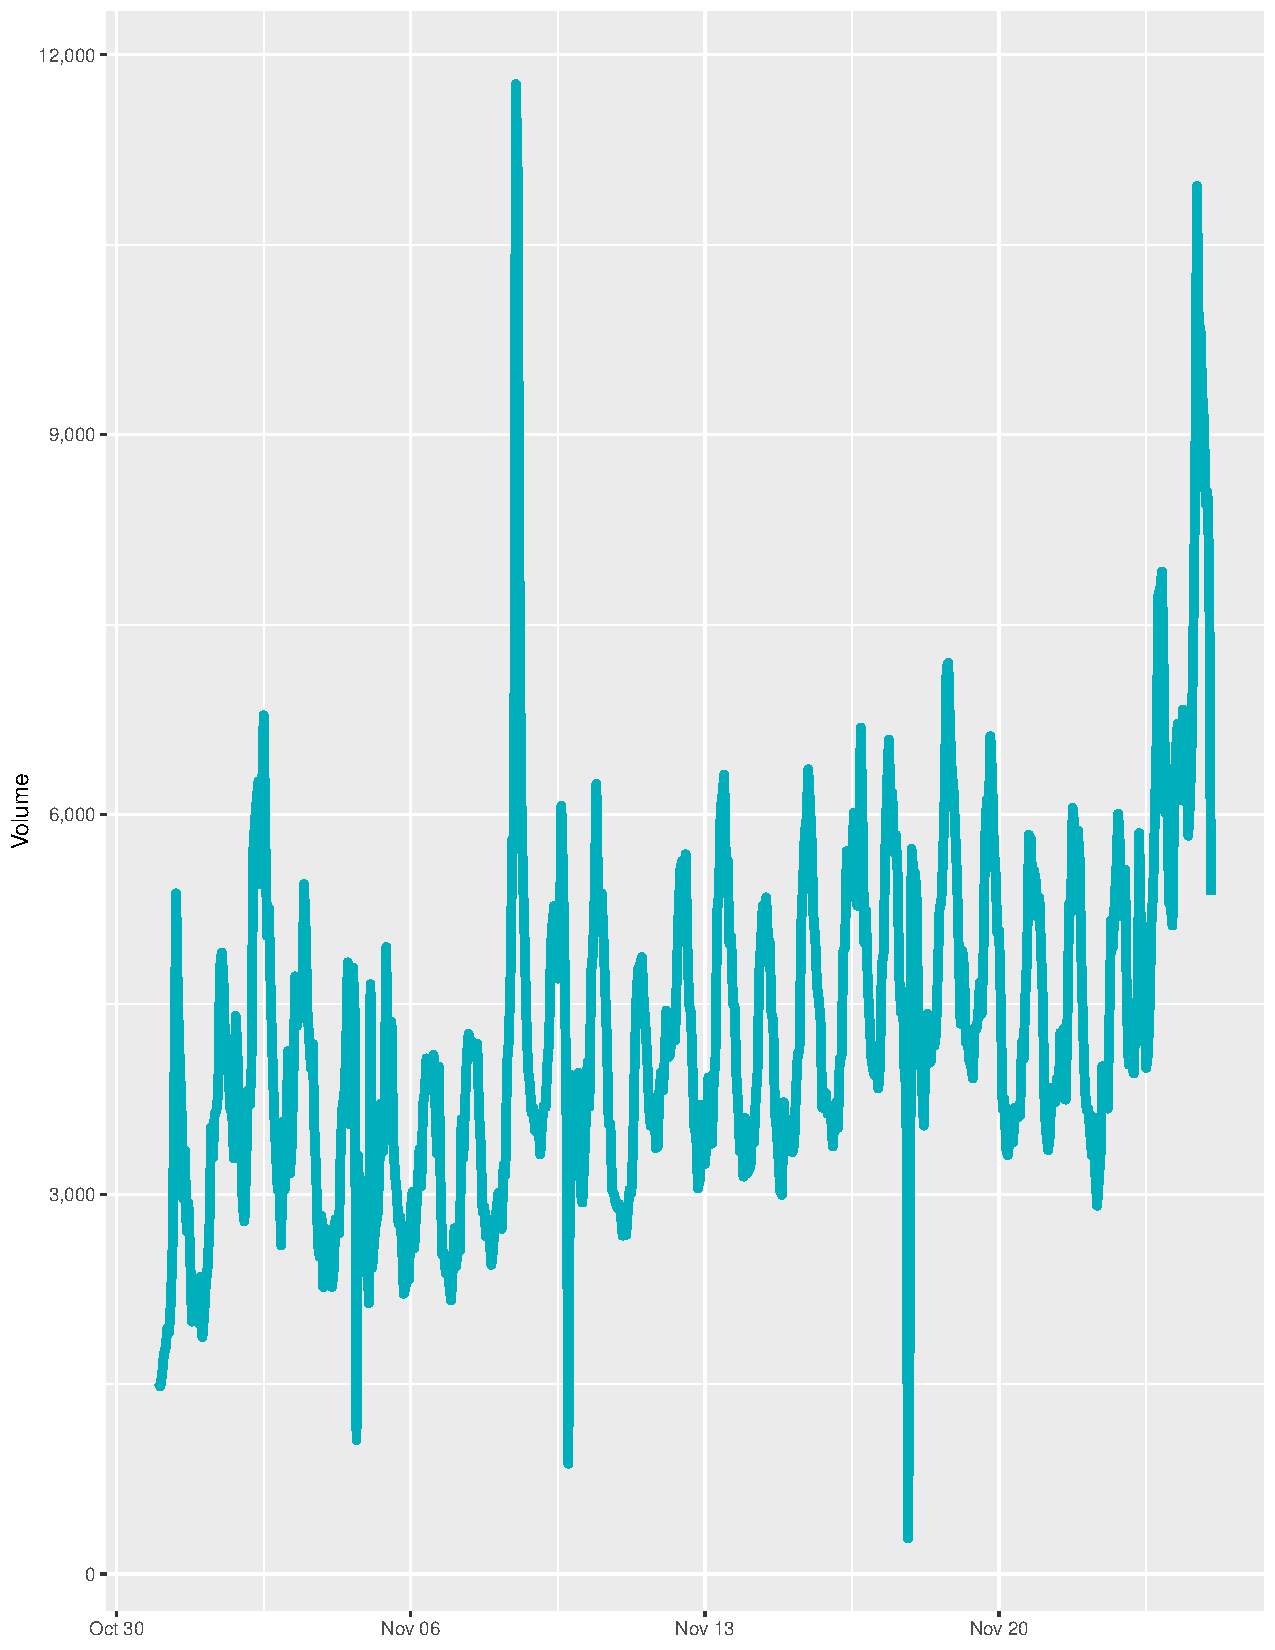
\includegraphics[scale=0.3]{Graphs/BitcoinVolumeChart.pdf}
\label{Bitcoin Volume Tweets} 
\end{figure}
\end{minipage}

\subsection{Pre-processing of the Tweets Data}
\par Tweets are pre-processed in order to filter out unnecessary data such as URLs. Moreover, they need to be converted into a feature vector representation. A number of preprocessing steps are taken.
\begin{enumerate}
\item \textit{Tokenization:} URLs are removed from the tweets. Often, tweets also consist of hashtags(\#) and of @ for addressing users, and they are removed consequently. In addition, all alphabetical characters are converted to lowercase. Tweets are then split and tokenized into individual words so that each tweet is then a list of words. Moreover, since LSTM will be used as a sentiment classifier and a uniformed input is needed for the model, tweets are then trimmed down to a maximum of 15 words.

\item \textit{Feature vector representation:} Word2vec is used in order to textually represent each tweet from their list of words. It allows for word embeddings where the meaning of the words are then sustained across different contexts, making the feature vector representation robust. A word2vec model is trained over a corpus of 1,578,612 tweets.
\end{enumerate}

\subsection{Sentiment Analysis}
\par Because of the lack of annotated sentiment analysis of tweet data specific to the financial domain and of Bitcoin, and since the above corpus of 1,578,612 tweets used to build the word2vec model has already been annotated as being either positive or negative, the corpus of tweets is also used to train a LSTM model that will then perform a sentiment analysis on the Bitcoin tweets. 80\% of the corpus tweets are used as the training set and the remaining 20\% as the test set. The choice of word2vec model is in particular appropriate in labelling the Bitcoin tweets since the embedded word representations trained through the corpus are valid across different contexts. The sentiment analysis outputs from the LSTM classifier on the Bitcoin tweets are grouped together according to their respective tweets occurrence in the hourly time frame, and an average is then performed so that every hour from the time period of October 31, 2017 till November 27, 2017 has an average public sentimental representation.  

\subsection{Long Short-Term Memory (LSTM)}
\par The LSTM is a type of recurrent neural network (RNN). Recurrent neural networks are suitable for sentiment analysis since they can establish long-term dependencies between data that are far apart and utilize contextual information. However, most recurrent neural networks have the critical problem of vanishing and exploding gradients. In order to fix this, Hochreiter and Schmidhuber \cite{LSTM} introduced the LSTM model, where memory cells are introduced to the memory blocks of the hidden layer of a RNN to allow the model to keep or to forget information. This is appropriate in a sentiment analysis tasks, since the use of LSTM may focus more on the important words. In fact, the LSTM is also appropriate as a time series model, since the use of long-term dependencies permits to learn nonlinear statistical dependencies of time series. As such, two LSTMs are used to learn on the two time series datasets of the Bitcoin prices, and of the volume of tweets respectively. For both of the datasets, the data for the next hour is predicted according to the sequence of data from the last 24 hours as inputs to the LSTM. Each of the LSTMs are built with one hidden layer.

\subsection{LSTM ensemble}
\par A LSTM ensemble is built by linearly combining the output of each of the LSTM models to output a final forecast for the price of Bitcoin. The ensemble can be interpreted as a mean to fine-tune the initial forecast of the price with additional information. Weights are assigned to the multiple LSTM models to produce the composite prediction output. That is, for a total of three LSTM models in the ensemble, representing each the historical prices, the volume of tweets and their sentiment analysis respectively, their ensemble forecast result for time series, denoted as $(y^{(1)}, \dots. y^{(N)})$ with $N$ overvations, is given by 

\begin{equation}
\label{LSTM ensemble weights}
\hat{y}^{(n)} = \sum_{i = 1}^{3} \omega_{i} \hat{y}_{i}^{(n)} ~, 
\end{equation} 
for $n = 1, \dots, N$.\\
$\hat{y}^{(n)}$ denotes the forecast output at time $n$ obtained by combining the three LSTM models with the associated weight $\omega_{i}$.
\par The proposed idea is that Bitcoin prices should reflect its past trend, while also considering its popularity among the public and of the latter sentiment towards it respectively. Figure \ref{Project Plan} summarizes the methodology used in this paper to predict the Bitcoin prices.

\begin{minipage}{\linewidth}
\begin{figure}[H]
\centering
\caption{The Proposed Model for Bitcoin Price Prediction} 
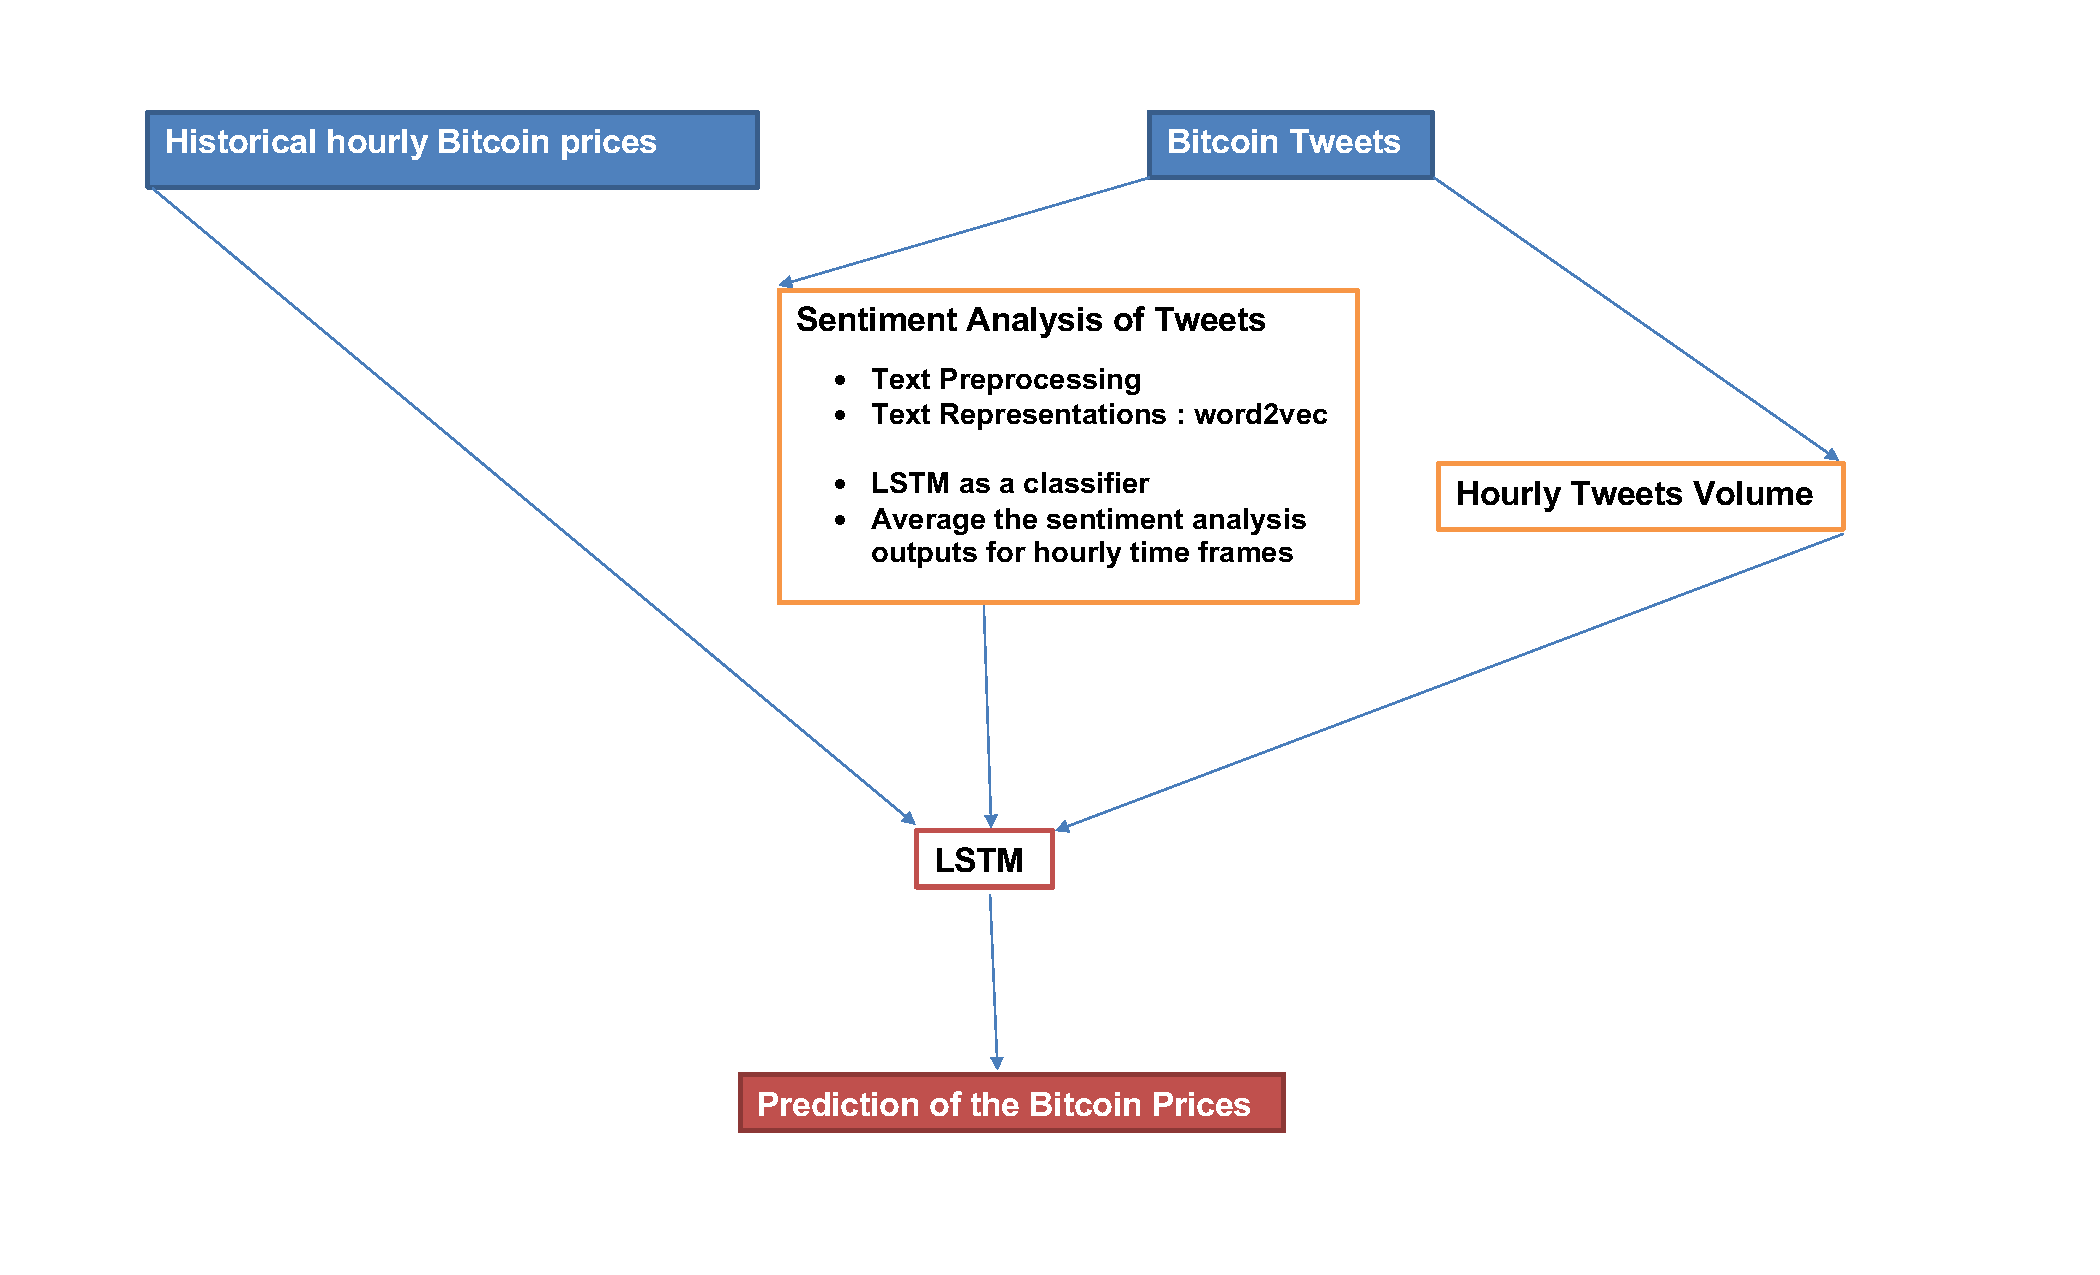
\includegraphics[scale=0.28]{Graphs/PlanProject.pdf}
\label{Project Plan} 
\end{figure}
\end{minipage}

\section{Results}
\par As discussed earlier, after training a word2vec model on the corpus of 1,578,612 tweets, a LSTM classifier feeding on the corpus is built to classify the sentiment of tweets. An accuracy of 0.7848 is achieved on the test set. Also shown is the associated ROC curve obtained from the different possible values of the decision boundary as it varies from 0 to 1 to classify the tweets as being negative or positive. Considering that the ROC curve is far over the random guesses curve, the model has good predictive power. Indeed, the random guesses curve represents what the ROC curve would look like if the model had no predictive power and would make random guesses. In fact, the idea behind an ROC curve is that the higher the area under the curve, the better prediction power the model has. The area under the curve is used to determine the predictive power of a classification model. For the model specified previously, the area under the curve corresponds to 0.87. This is considered to have good predictive power for a classification model.

\begin{minipage}{\linewidth}
\begin{figure}[H]
\centering
\caption{ROC curve for the LSTM classifier of tweets} 
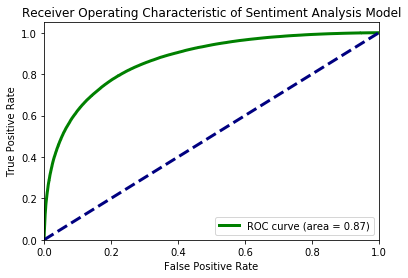
\includegraphics[scale=0.4]{Graphs/ROCCurveSentiment.png}
\label{ROC Sentiment} 
\end{figure}
\end{minipage}


\begin{thebibliography}{2}
\bibitem{LSTM Ensemble 1} Choi, JY.; Lee, B.. Combining LSTM network ensemble via adaptive weighting for improved time series forecasting. \textit{Math. Problems Eng.,}, \textbf{2018}, Art. no. 2470171.

\bibitem{Behavior} Khedr, A.E.; Salama, S.E.; Yaseen, N. Predicting Stock Market Behavior using Data Mining Technique and News Sentiment Analysis. \textit{Int. J. Intell. Syst. Appl.} \textbf{2017}, 7, 22-30.

\bibitem {LSTM} Sepp Hochreiter and Jurgen Schmidhuber. Long short-term memory. \textit{Neural Comput.}, \textbf{1997}, 9(8):1735-1780
\bibitem{LSTM Stock} Nelson, D. M. Q.; Pereira, A. C. M.; de Oliveira, R. A.. Stock market’s price movement
prediction with LSTM neural networks. \textit{International Joint Conference on Neural Networks (IJCNN)}, \textbf{2017}, 1419-1426.

\bibitem{word2vec Twitter} Pagolu, V. S.; Reddy, K. N.; Ganapati Panda; Majhi, B.. Sentiment
analysis of twitter data for predicting stock market
movements. \textit{International
Conference on Signal Processing, Communication,
Power and Embedded System}, \textbf{2016}, 1345-1350.

\bibitem{LSTM Emotional} Zhuge, Q.; Xu, L.Y.; Zhang, G.W..  LSTM Neural Network with Emotional
Analysis for Prediction of Stock Price. \textit{Engineering Letters}, \textbf{2017}, 25, 167-175.

\bibitem{Twitter API} https://dev.twitter.com/overview/api
\end{thebibliography}




\end{document}
